%\chapter{Balancing Map Compression with Sensing Accuracy}
\chapter{}
\label{chapter4}

The PRI strategy in Sec.~\ref{subsec:pri} determines an optimal compression given a desired OG resolution. However, Fig.~\ref{fig:csqmi_timing} suggests that one should also reduce the resolution of the OG as much as possible to increase efficiency. In this section we formulate a second optimization based on the Information Bottleneck (IB) method~\cite{tishby2000information} that chooses a grid resolution minimizing both the redundancy between $m^{K}$ and
$C_{n}(m^{K})$, and loss of mutual information with respect to a sensor measurement $z$.


\section{The Information Bottleneck Method}

IB is a widely used technique in signal processing for finding the optimal reduced representation $\hat{X}$ of a random variable $X$ that preserves maximum information about a second random variable $Y$:
%
\eq{
    \min_{\hat{X}}
    \text{I}(X; \hat{X})
    -
    \beta
    \text{I}(\hat{X}; Y).
    \label{eq:ib_opt}
}

IB resembles PRI, but considers the effects of compression on the information between two datasets, as opposed to one. Similar to $\lambda$ in the PRI optimization, $\beta$ is a design parameter that trades compression for conservation of information. As $\beta \rightarrow 0$, the optimization tends towards the trivial lossy compression $\{\hat{X}\}=0$, whereas when $\beta \rightarrow \infty$, $\hat{X}$ approaches its original representation $X$~\cite{principe2010information}. The two terms in the argument of~\eqref{eq:ib_opt} can equivalently be thought of as the information loss incurred by describing $\hat{X}$ with $Y$ instead of with $X$~\cite{geiger2011information}.

Most importantly for OG compression, when combined with the PRI approach in Section~\ref{subsec:pri}, the IB method can be used to find an optimal compression $n^{*}$:
%
\begin{gather}
    n^{*}
    =
    \argmin_{
        n \in \mbb{N}_{0}
    } \, \,
    \text{I}_{\text{CS}}\left(m^{K}; C_{n}(m^{K})\right)
    -
    \beta
    \text{I}_{\text{CS}}\left(C_{n}(m^{K}); z\right).
    \label{eq:ib_arg_opt}
\end{gather}

\section{Optimizing Map Resolution for Sensing}

\begin{sidewaystable*}[Ht!]
  \caption[A contingency table for occupancy grid compression
  distributions.]{Contingency table for a compression from the OG region
  $\mbf{m}^{R}$ to $\tilde{\mbf{m}}^{R}$. \texttt{O} and \texttt{E} stand for \texttt{OCC} and \texttt{EMP}. \label{tab:contingency}}
    \centering
    \scalebox{0.9}
    {
    \renewcommand{\arraystretch}{3}
    \begin{tabular}{| c | c | c | c | c | c | c | c |}
        \cline{3-7}
        \multicolumn{2}{c|}{}
        & \multicolumn{1}{c}{}
        & \multicolumn{1}{c}{}
        & \multicolumn{1}{c}{$\tilde{\mbf{m}}^{R}$}
        & \multicolumn{1}{c}{}
        & \multicolumn{1}{c|}{}
        & \multicolumn{1}{c}{}
        \\ \cline{3-8}
        \multicolumn{2}{c|}{}
        & \scalebox{0.9}{\texttt{E}, \texttt{E}, $\dots$, \texttt{E}} & \scalebox{0.9}{\texttt{E}, \texttt{E}, $\dots$, \texttt{O}} & $\dots$ & \scalebox{0.9}{\texttt{O}, \texttt{O}, $\dots$, \texttt{E}} & \scalebox{0.9}{\texttt{O}, \texttt{O}, $\dots$, \texttt{O}} & Total \\ \cline{1-4}\cline{6-8}
        \multirow{5}{*}{$\mbf{m}^{R}$}
        & \scalebox{0.9}{\texttt{E}, \texttt{E}, $\dots$, \texttt{E}} &
        $w_{2}\cdot(1-\tilde{\mbf{o}}^{1}) \cdot
        \prod_{i=1}^{R}(1-\mbf{o}_{i}^{R})$ & $0$ & $\dots$ & $0$ & $w_{3}\cdot
        \tilde{\mbf{o}}^{1}\cdot \prod_{i=1}^{R}(1-\mbf{o}_{i}^{R})$ &
        $\prod_{i=1}^{R}(1-\mbf{o}_{i}^{R})$\\ \cline{2-4}\cline{6-8}
        & \scalebox{0.9}{\texttt{E}, \texttt{E}, $\dots$, \texttt{O}} &
        $w_{1}\cdot(1-\tilde{\mbf{o}}^{1})\cdot \mbf{o}_{1}^{R}\cdot
        \prod_{i=2}^{R}(1-\mbf{o}_{i}^{R})$ & $0$ & $\dots$ & $0$ &
        $w_{4}\cdot\tilde{\mbf{o}}^{1}\cdot \mbf{o}_{1}\cdot
        \prod_{i=2}^{R}(1-\mbf{o}_{i}^{R})$ & $\mbf{o}_{1}\cdot
        \prod_{i=2}^{R}(1-\mbf{o}_{i}^{R})$\\ \cline{2-4}\cline{6-8}
        &
        \multicolumn{1}{c}{$\vdots$}
        &
        \multicolumn{1}{c}{$\vdots$}
        &
        \multicolumn{1}{c}{$\vdots$}
        &
        \multicolumn{1}{c}{$\ddots$}
        &
        \multicolumn{1}{c}{$\vdots$}
        &
        \multicolumn{1}{c}{$\vdots$}
        &
        \multicolumn{1}{c|}{$\vdots$} \\ \cline{2-4}\cline{6-8}
        & \scalebox{0.9}{\texttt{O}, \texttt{O}, $\dots$, \texttt{E}} & $ w_{1}
        \cdot (1-\tilde{\mbf{o}}^{1})\cdot (1-\mbf{o}_{1}^{R}) \cdot
        \prod_{i=2}^{R} \mbf{o}_{i}^{R}$ & $0$ & $\dots$ & $0$ & $w_{4}\cdot
        \tilde{\mbf{o}}^{1}\cdot (1-\mbf{o}_{1}^{R}) \cdot \prod_{i=2}^{R}
        \mbf{o}_{i}^{R}$ & $(1-\mbf{o}_{1}^{R}) \cdot \prod_{i=2}^{R} \mbf{o}_{i}^{R}$\\ \cline{2-4}\cline{6-8}
        & \scalebox{0.9}{\texttt{O}, \texttt{O}, $\dots$, \texttt{O}} &
        $w_{1}\cdot(1-\tilde{\mbf{o}}^{1})\cdot \prod_{i=1}^{R}\mbf{o}_{i}^{R}$
        & $0$ & $\dots$ & $0$ & $w_{4}\cdot\tilde{\mbf{o}}^{1}\cdot
        \prod_{i=1}^{R}\mbf{o}_{i}^{R}$ & $\prod_{i=1}^{R}\mbf{o}_{i}^{R}$ \\ \cline{1-4}\cline{6-8}
        \multicolumn{1}{c|}{}
        & Total & $1-\tilde{\mbf{o}}^{1}$ & $0$ & $\dots$ & $0$ &
        $\tilde{\mbf{o}}^{1}$ & 1 \\ \cline{2-8}
    \end{tabular}
    }
\end{sidewaystable*}



The second term can be computed using~\eqref{eq:csqmi}, and is $2^{1\times n}$ times more efficient than computing~\eqref{eq:csqmi} with respect to the uncompressed map $m^{K}$ (where $d=1$ because $\text{I}_{\text{CS}}(m;z_{\tau})$ is computed using 1D raycasts). Since $\text{I}_{\text{CS}}(m^{K};C_{n}(m^{K}))$ describes the divergence between the distributions $p(m^{K},C_{n}(m^{K}))$ and $p(m^{K})p(C_{n}({m}^{K}))$, the first term in~\eqref{eq:csqmi} can be computed by substituting these for $p(x_i)$ and $p(\hat{x}_{i})$ in the definition of Cauchy-Schwarz divergence~\eqref{eq:cs_divergence}.

However, the joint distribution $p(m^{K},C_{n}(m^{K}))$ is underdetermined by two variables, and must be constrained before computing~\eqref{eq:ib_arg_opt}. While the remaining two degrees of freedom make the IB cost function arbitrary for a single resolution, fixing the joint distribution and using it to compute CSQMI across different grid resolutions still yields a meaningful optimization. To constrain the extra degrees of freedom we first decompose the joint distribution into independent regions $r \in m^{K}$:
%
\eq{
p(m^{K},C_{n}(m^{K}))
&=
\prod_{r \in m^{K}}
p(m^{R}_{r},C_{n}(m^{R}_{r})) \\
&=
\prod_{r \in m^{K}}
p(m^{R}_{r},\tilde{m}^{R}_{r}),
}

where the second equation holds by noting $C_{n}(m^{R}_{r})$ has a dimension of one, and that that all cells in $\tilde{m}^{r}$ are completely determined by knowing $C_{n}(m^{R}_{r})$. Then, for each region $r$, we choose the joint distribution $p(m^{R}_{r},\tilde{m}^{R}_{r}))$ to be a product of the marginals $p(m^{R}_{r})$ and $p(\tilde{m}^R_{r}))$, weighted by four extra coefficients $w_{1:4}$ (Table~\ref{tab:contingency}). Similar to the reasons that $\eta$ in Sec.~\ref{subsec:pri} is chosen to preserve occupied cells through compression, the constant $c_1 \in (0, 1)$ downweighs the probability of the event that $\tilde{m}^{R}$ is $\{\texttt{EMP},\dots,\texttt{EMP}\}$ if any grid cells in $m^{R}$ are occupied. The remaining three constants balance the effects of $w_{1}$ such that the conditional distributions over the rows and columns of Table~\ref{tab:contingency} all sum to the marginal distributions on the bottom-most row and right-most column.

%the first term can be computed by substituting $p(m^{K},C_{n}(m^{K}))$ and $p(m^{K})p(C_{n}({m}^{K}))$ for $p(x_i)$ and $p(\hat{x}_{i})$ in~\eqref{eq:cs_divergence}, respectively. However, the joint distribution $p(m^{K},C_{n}(m^{K}))$

%derivation in Sec.~\ref{subsec:pri} left the joint distribution $p(m^{R},\,\tilde{})$


%the first term cannot immediately be evaluated because the PRI compression derivation leaves the joint distribution $p(m^{R}, \tilde{m}^{R})$ underconstrained. While the remaining two degrees of freedom make the IB cost function arbitrary for a single resolution, fixing the joint and using it to compute CSQMI across different grid resolutions still yields a meaningful optimization. We choose the joint to be a product of the marginals $p(m^{R})$ and $p(\tilde{m}^{R})$, weighted by four extra coefficients $w_{1:4}$. Just as $\eta$ in Sec.~\ref{subsec:pri} is chosen to preserve occupied cells through compression, the constant $c_1 \in (0, 1)$ downweighs the probability of the event that $\tilde{m}^{R}$ is $\{\texttt{EMP},\dots,\texttt{EMP}\}$ if any grid cells in $m^{R}$ are occupied. The remaining three constants balance the effects of $w_{1}$ such that the conditional distributions in the rows and columns of Table~\ref{tab:contingency} all sum to the marginals. With the joint distribution fixed, the first term in~\eqref{eq:ib_arg_opt} can be computed by substituting $p(m^{R},\tilde{m}^{R})$ and $p(m^{R})p(\tilde{m}^{R})$ for $p(x_i)$ and $p(\hat{x}_{i})$ in~\eqref{eq:cs_divergence}, respectively.

Figure~\ref{fig:loss_compression} displays the influence of $\beta$ on the IB optimization for a multi-beam measurement captured from a planned future location. The optimization favors no compression when $\beta$ is large, and maximum compression when $\beta$ is small.

\begin{figure}
    \centering
    \begin{subfigure}[t]{0.45\textwidth}
        \centering
        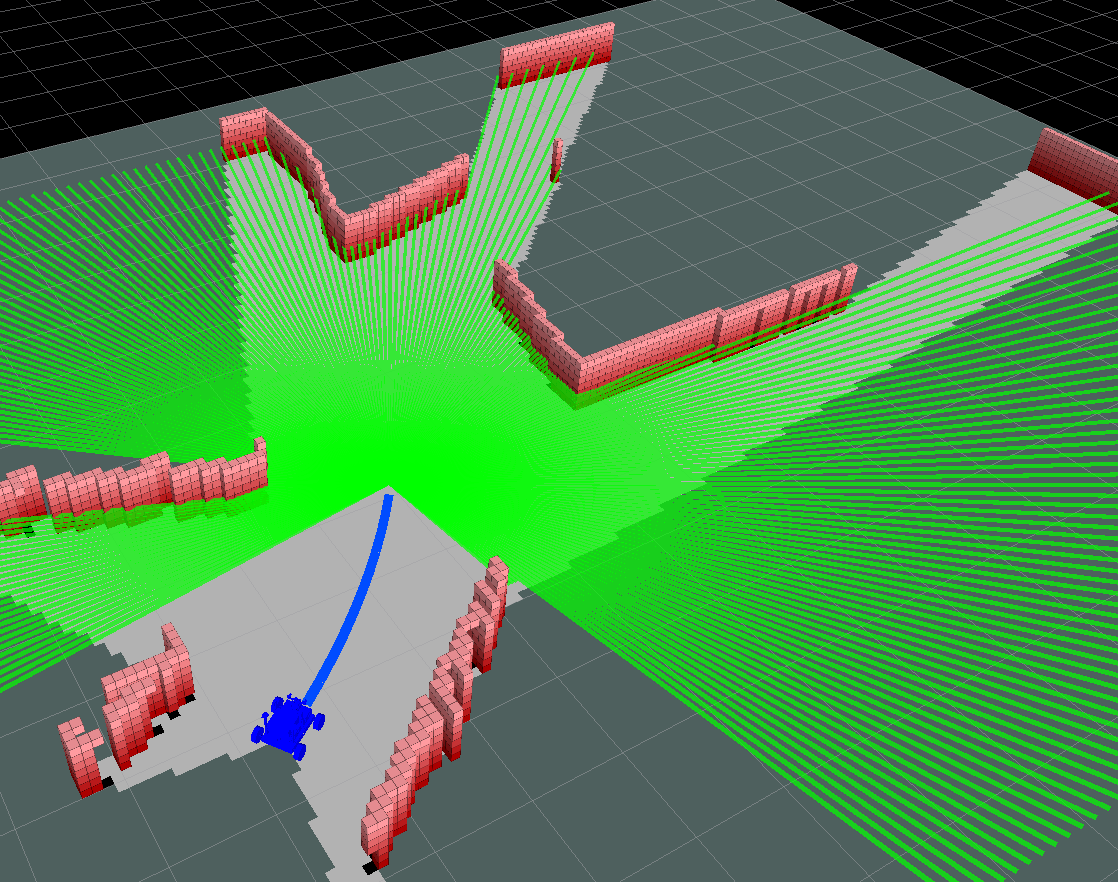
\includegraphics[height=6cm]{plan_ahead.png}
        \caption{\label{fig:loss_compression1}}
    \end{subfigure}
    \hfill
    \begin{subfigure}[t]{0.45\textwidth}
        \centering
        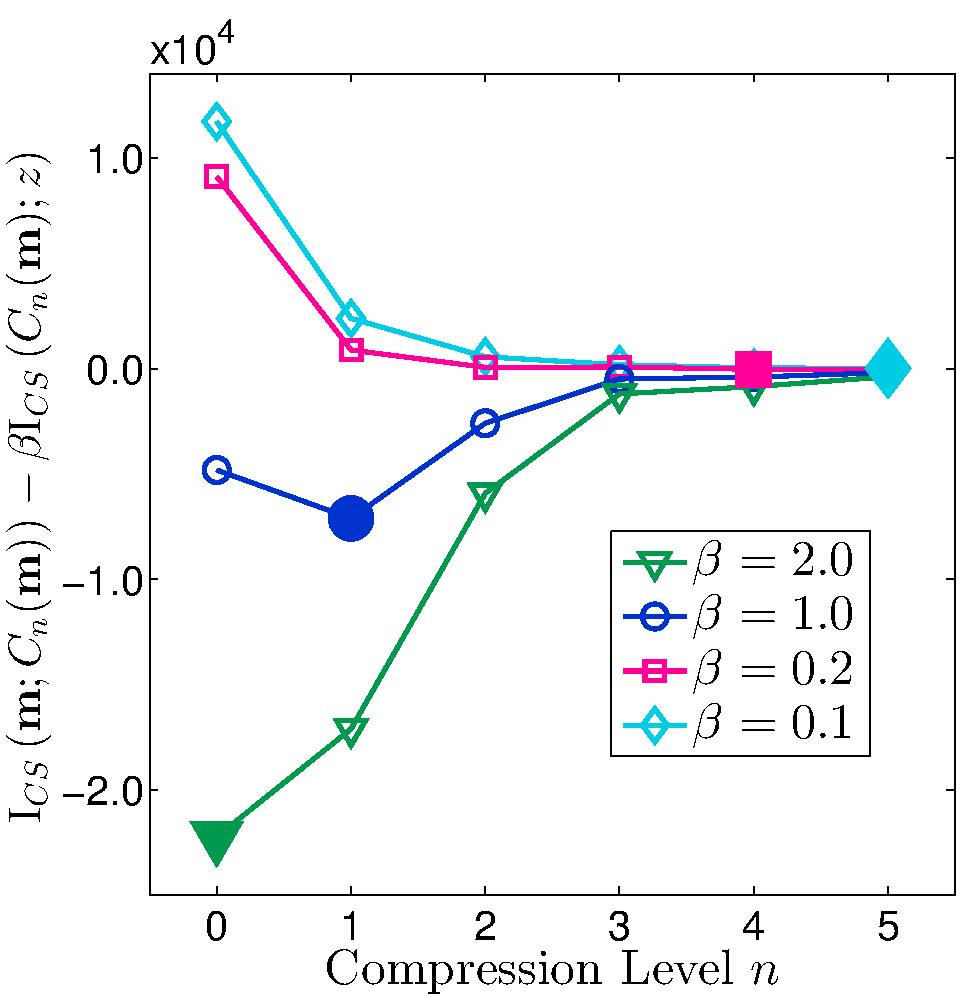
\includegraphics[height=6.5cm]{beta.pdf}
        \caption{\label{fig:loss_compression2}}
    \end{subfigure}
    \caption[Information Bottleneck optimization for varying values of $\beta$]{\ref{fig:loss_compression1} shows an uncompressed map and measurement taken from a planned future position. With this map and expected laser scan, the optimal compression level (filled markers) computed with~\eqref{eq:ib_arg_opt} decreases as $\beta$ increases, favoring preservation of information about the measurement as opposed to compression (\ref{fig:loss_compression2}). \label{fig:loss_compression}}
\end{figure}

\section{Results}

\begin{figure}
  \centering
  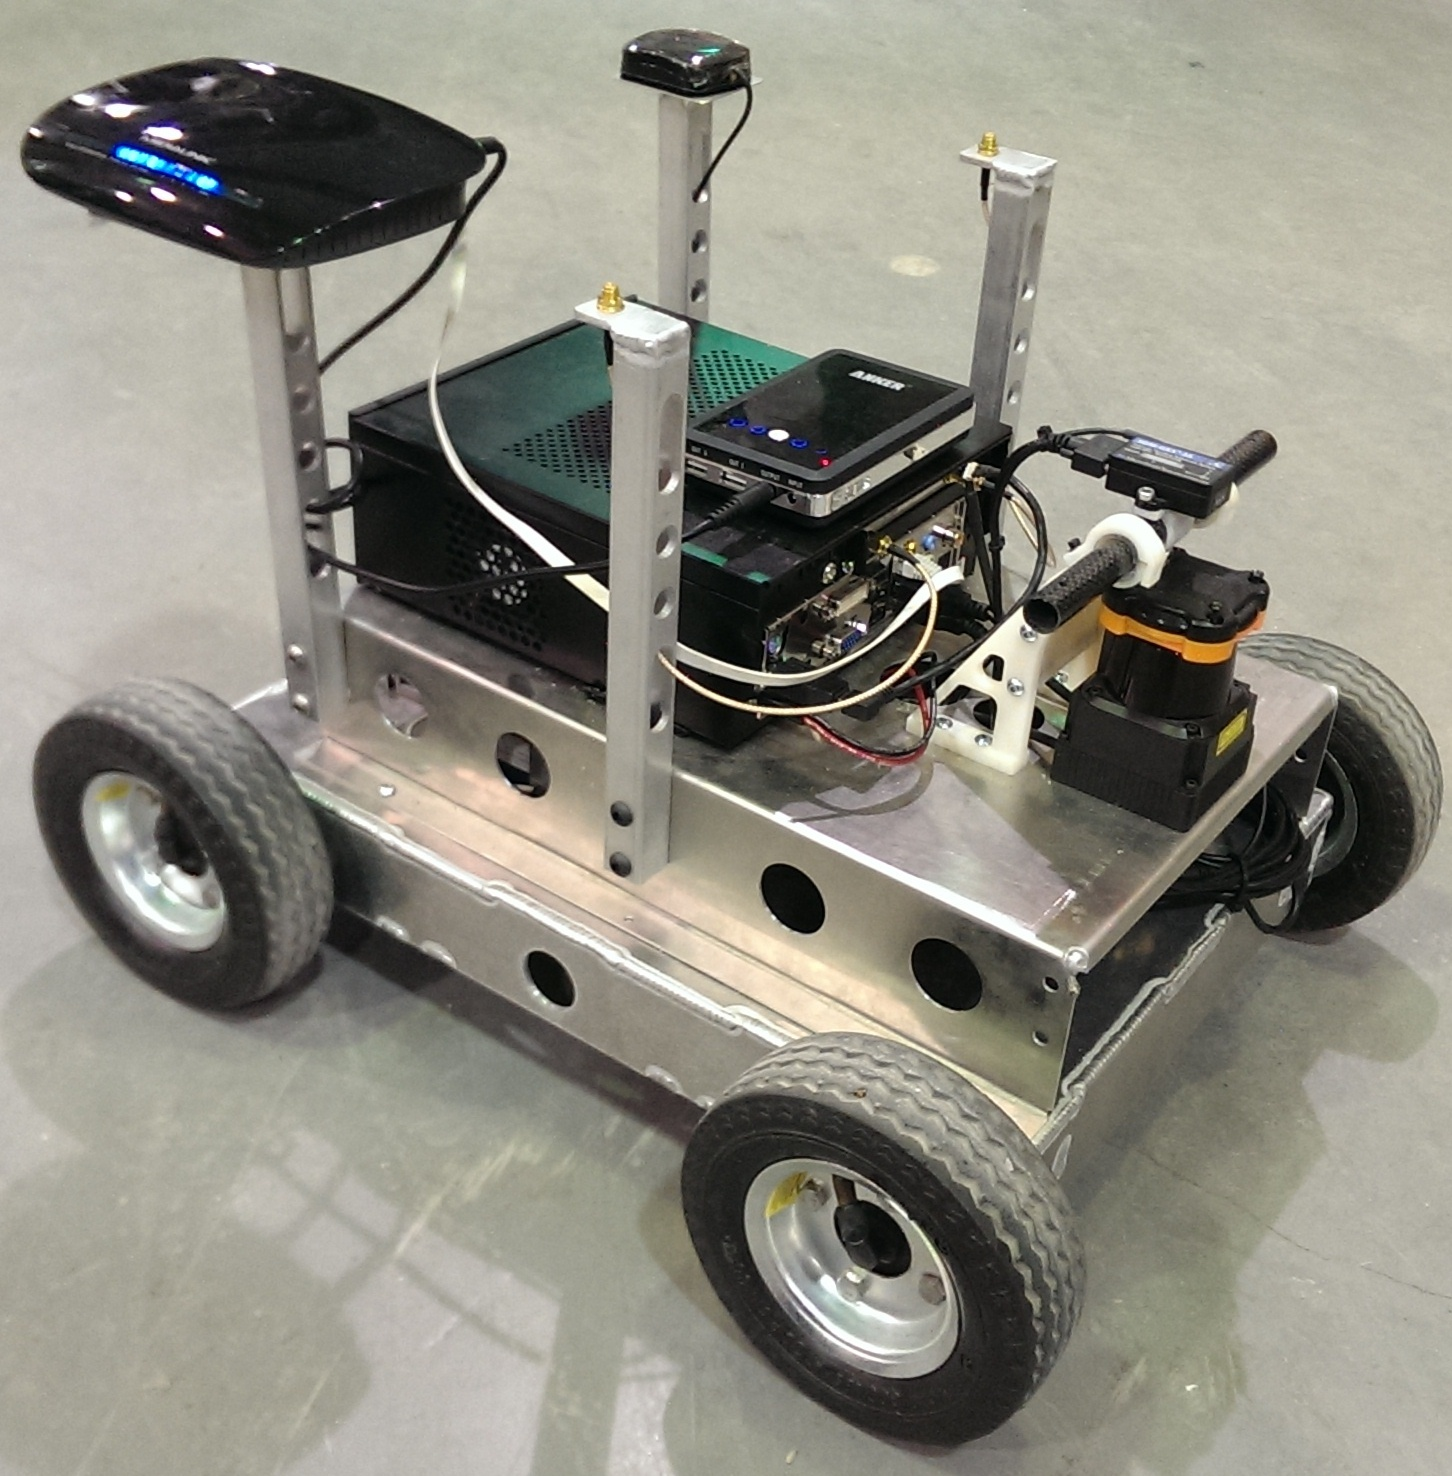
\includegraphics[width=0.6\textwidth]{groundbot.jpg}
  \caption{Robot Platform\label{fig:robot_platform}}
\end{figure}

\begin{figure}
  \centering
  \begin{subfigure}[t]{0.64\textwidth}
    \centering
    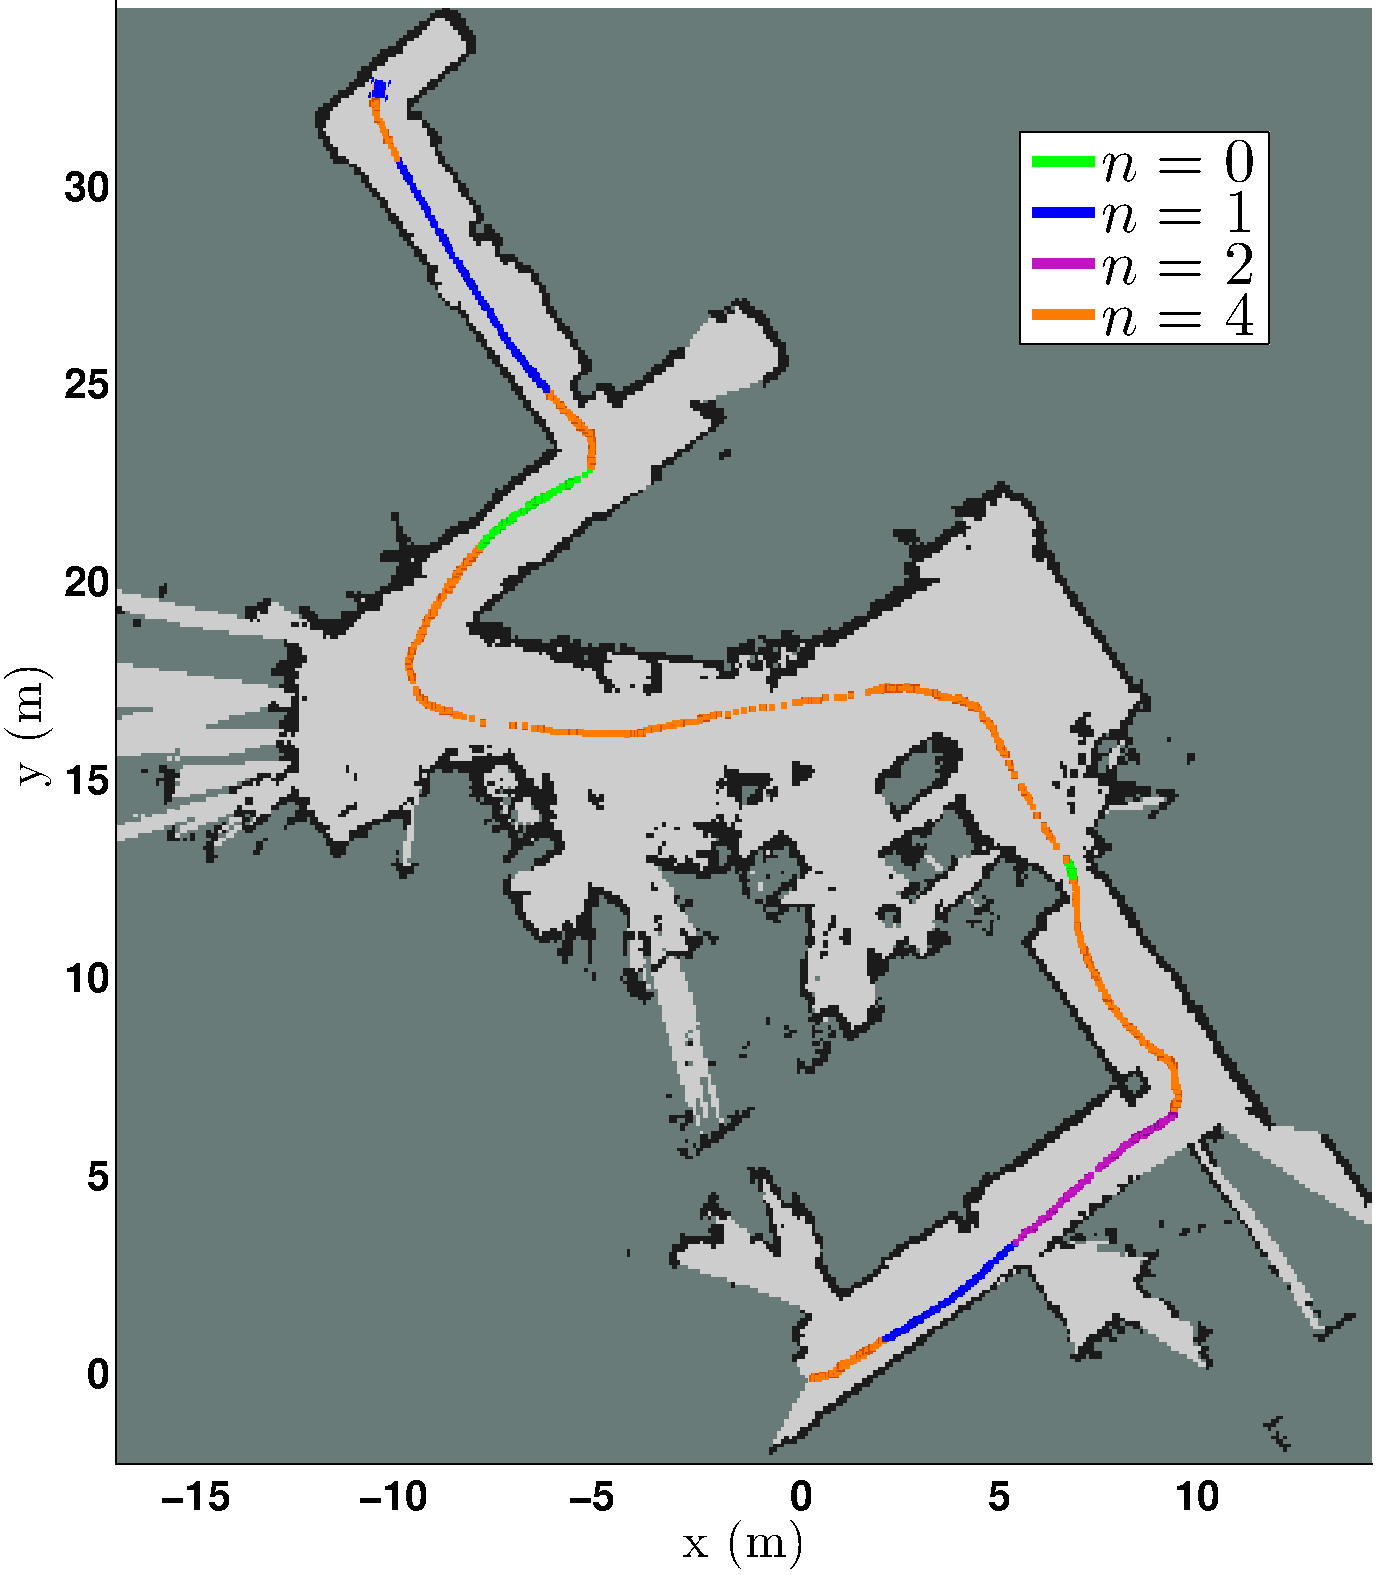
\includegraphics[width=\textwidth]{ground_experiment_map2.pdf}
    \caption{Exploration path \label{fig:ib_exploration_path}}
  \end{subfigure}
  \\
  \begin{subfigure}[t]{0.8\textwidth}
    \centering
    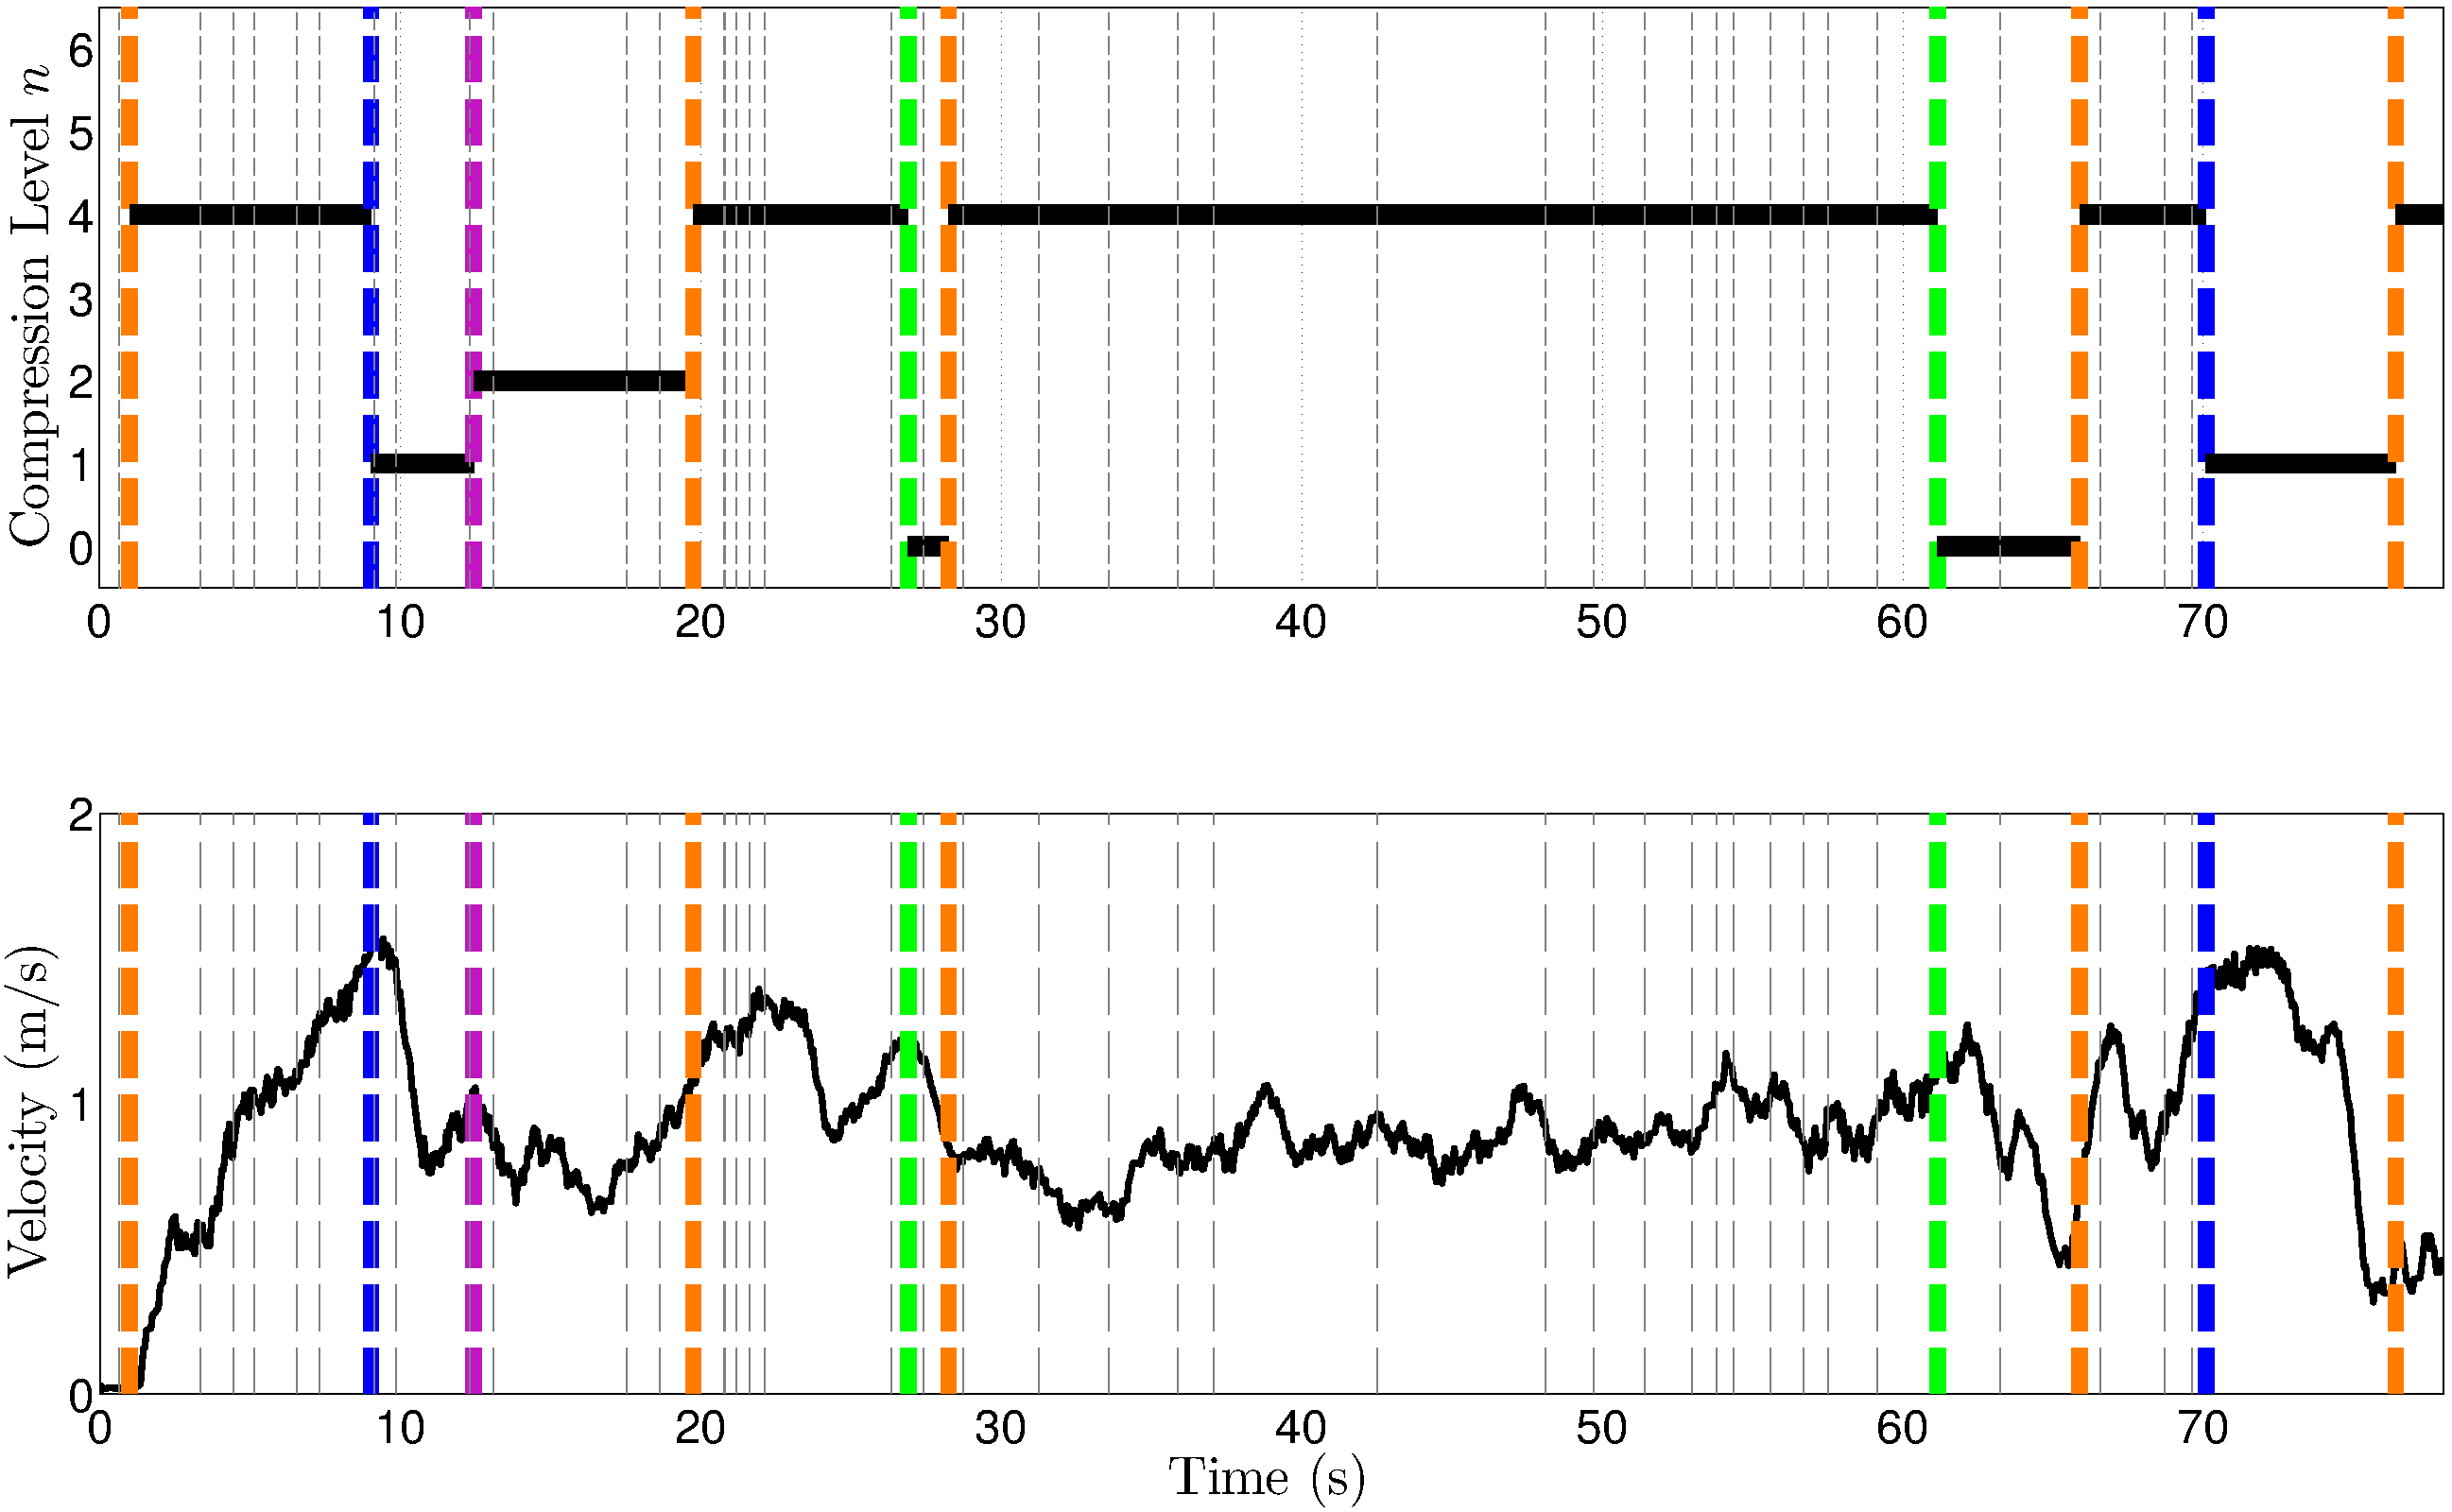
\includegraphics[width=\textwidth]{ground_experiment.pdf}
    \caption{Time evolution of $n$ and velocity.\label{fig:ib_exploration_plots}}
  \end{subfigure}
  \caption{As the ground robot explores, it recomputes an optimal OG resolution and adapts its dynamics accordingly.\label{fig:ground_experiment}}
\end{figure}



\section{Chapter Summary}
